\documentclass[tikz,border=2mm]{standalone}
\usepackage{tikz}
\usetikzlibrary{automata,positioning}
\begin{document}
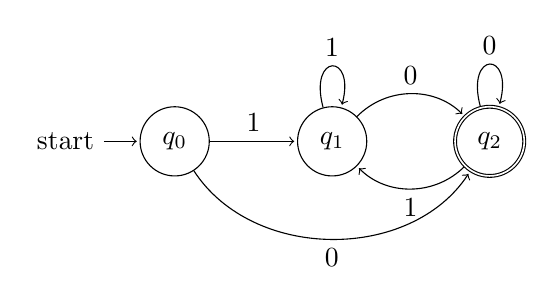
\begin{tikzpicture}[shorten >=1pt,node distance=2cm,on grid,auto,bend angle=45] 

  \node[state,initial] (q_0)  {$q_0$};
  \node[state] (q_1) [right=of q_0] {$q_1$};
  \node[state,accepting] (q_2) [right=of q_1] {$q_2$};

  \path[->]
    (q_0) edge[above] node{1} (q_1)
    (q_0) edge[bend right=2cm, below] node{0} (q_2)
    (q_1) edge[loop above] node{1} (q_1)
    (q_1) edge[bend left, above] node{0} (q_2)
    (q_2) edge[loop above] node{0} (q_2)
    (q_2) edge[bend left, below] node{1} (q_1);



\end{tikzpicture}
\end{document}  
